\documentclass[conference]{IEEEtran}
\usepackage{multirow}
\usepackage{array}
\usepackage[loftdepth, lotdepth]{subfig}
\usepackage{color}
\usepackage{amssymb}
\usepackage{booktabs}
\usepackage{rotating}
\usepackage{amsmath}
\usepackage{wrapfig}
\usepackage{algorithm}
\usepackage{algpseudocode}
\usepackage{lineno,hyperref}
\usepackage{graphicx}
\usepackage{biblatex}
\addbibresource{reference.bib}
\usepackage{mathtools}

\usepackage{pdflscape}
\usepackage[none]{hyphenat}
%\usepackage[latin1]{inputenc}
\providecommand{\keywordss}[1]{\textbf{\textit{Anahtar Kelimeler---}} #1}
\providecommand{\keyword}[1]{\textbf{\textit{Keywords---}} #1}
\providecommand{\ozet}[1]{\textbf{\textit{Özetle---}} #1}
\providecommand{\summary}[1]{\textbf{\textit{İn Summary---}} #1}
\providecommand{\abstracts}[1]{\textbf{\textit{Abstract---}} #1}
\usepackage[utf8]{inputenc}

\begin{document}
\large

\title{Yapay Zeka Temelli Kalp Yetmezliği Teşhisi\\
Artificial Intelligence Based Heart Failure Diagnosis
}

\author{
\IEEEauthorblockN{Hüseyin TAŞ}
\IEEEauthorblockA{Bilgisayar Mühendisliği\\
    Kahramanmaraş Sütçü İmam Üniversitesi\\
    Kahramanmaraş,Türkiye\\
    htas19318@gmail.com
}
\and
\IEEEauthorblockN{Muhsin DENİZ}
\IEEEauthorblockA{Bilgisayar Mühendisliği\\
    Kahramanmaraş Sütçü İmam Üniversitesi\\
    Kahramanmaraş,Türkiye\\
    mnknsro413@gmail.com
}
}
\date{January 2022}
\maketitle
\begin{ozet}
Kalp yetmezliği hastadan toplanan çeşitli veriler ile  teşhis edilebilmektedir. Bu veriler hastaya belirli testler uygulayarak elde edilir. Hastadan elde edilen verilere bir sınıflandırma algoritması uygulayarak kalp hastalığı teşhis edilebilmektedir.Bu çalışmada problemin çözümü için Yapay sinir ağları ve K en yakın komşu algoritması önerilmiştir. Önerilen yöntem, yaygın olarak kullanılan  Lojistik regresyon(logistic regression),Rastgele orman(random forest) ve K en yakın komşu(K nearest neighbors) gibi sınıflandırma algoritmaları ile karşılaştırmalı olarak analiz edilmiştir.\\
\end{ozet}
\begin{keywordss}
Kalp yetmezliği, Yapay sinir ağları\\
\end{keywordss}

\begin{abstracts}
Heart failure can be diagnosed with various data collected from the patient. These data are obtained by applying certain tests to the patient. Heart disease can be diagnosed by applying a classification algorithm to the data obtained from the patient. In this study, artificial neural networks and K nearest neighbor algorithm are proposed to solve the problem. The proposed method is comparatively analyzed with classification algorithms such as logistic regression,random forest and k nearest neighbors.\\
\end{abstracts}
\begin{keyword}
Heart failure, Artificial neural network
\end{keyword}

\section{GİRİŞ}
Kardiyovasküler hastalıklar dünyadaki ölümlerin 1 numaralı sebebidir. Kardiyovasküler hastalıklar kalp ve damar hastalıklarını kapsamaktadır. Kardiyovasküler hastalığı olan veya yüksek kardiyovasküler risk altında olan kişiler hipertansiyon, diyabet, hiperlipidemi veya halihazırda yerleşik hastalık gibi bir veya daha fazla risk faktörünün varlığı nedeniyle, hastalığın erken tespitine ve yönetimine ihtiyaç duyar\cite{kaggle}.\\

Kalp yetmezliği kardiyovasküler hastalıklar grubuna girer ve bu hastalık grubunda gerçekleşen ölümlerin çoğu bu kalp yetmezliğinden kaynaklanmaktadır. Kalp yetmezliği, kalbin kanı tüm vücuda pompalayamaması sonucunda kalbte oluşan ritim bozuklukluğuna ve damarlarda daralmalara sebep olmaktadır. Bu durumda vücuda kan pompalayamadığından dolayı organlarda ve dokularda hasar meydana gelmektedir. Bu yüzden kalp yetmezliğinin erken teşhisi önemlidir.Kalp hastalarında boyundaki kan damarlarının belirginleşmesi, nabızda düzensizlik(aritmi), ani kilo artışı ve kalp çarpıntısı vb. belirtiler görülmektedir.\\

Kalp hastalığının teshişi için birkaç adımdan oluşan zorlu işlemler gerektirmektedir. Hastalara uygulanna testler sonucunda elde edilen veriler sıkıntılı olabilmektedir. Örneğin veri eksik veya test sonucu beklenmeyen değerler bulunabilmektedir. Bu yüzden verilerimizi gürültülerden arındırmalıyız. Daha sonra elde edilen verilere sınıflandırma algoritması uygulanarak hastalık teşhis edilir.\\

Bu çalışmada fedesoriano tarafından yayınlanan, kalp yetmezliğini teşhis etmede kullanılan 11 özniteliği bulunduran bir veri kümesini projemizde önerilen sınıflandırma algoritmaları kullanılarak, hastaların kalp yetmezliği riskinin olup olmadığını tespit etmek amaçlanmaktadır\cite{data_author}. Ayrıca projemizde önerilen yöntemler ile Yapay Sinir Ağları ve K-en Yakın Komşu algoritmalarını kullanarak sınıflandırma başarımız test edilmesi amaçlanmaktadır.

Çalışmamız literatürde kullanılan Lojistik regresyon, Rastgele orman,K en yakın komşu ve diğer makine öğrenmesi sınıflandırma algoritmaları ile modellenen modellerin başarı oranlarının karşılaştırılması amaçlanmaktadır.

\section{YÖNTEM}
Kalp yetmezliği hastalığı tespit edilemsi sürecinde, Şekil 1'de görülen çalışmamızın önrelen yöntemidir.
Önerilen yöntemde öznitelik sayısı 12 olan ve 918 satır örnek oluşturan bir veri üzerinde 2 farklı makine öğrenmesi algoritması ile kalp yetmezliği hastalığı teşhisi sınıflandırılması gerçekleştirilmiştir.
\begin{figure}[htbp]
    \centering
   	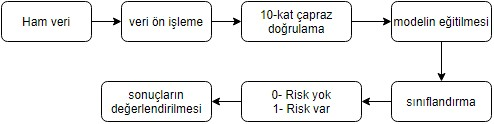
\includegraphics[width=8cm]{images/yontem.JPG}\\
	\caption{Kalp yetmezliği hastalığı teşhis etme aşamaları}
    \label{fig}
\end{figure}

Makine öğrenmesi bizim verdiğimiz veri setindeki veriler arasındaki ilişkiyi hesaplayan ve bunu bir matematiksel formüle oturtmaya çalışımaktadır. Daha sonra biz yeni bir veri verdiğimizde bunun hasta olup olmadığını tespit edebilmektedir. Veri ön işleme makine öğrenmesi modelini kurmadan önce veri setindeki aykırı değerleri kaldırma, eksik verileri düzenleme ve verileri dönüştürme gibi işlemleri kapsamktadır. Veri ön işleme aslında veri setini modele girebilmesi için hazır hale getirir. Veri ön işleme modelimizin başarısı için önemdlidir. Çünkü veri setinde eksik veri olursa veya aykırı veriler olursa bunlar modelin başarı oranını düşürmektedir. 

Önerilen yöntemdeki 10-kat çapraz doğrulama ise modelimizin doğruluk oranını sınamaktadır. Örneğin model oluşturmadan önce veri setini eğitim ve test veri seti olarak ayırdık ve modeli eğitim verisi ile eğitip test veris ile test edilmektedir. Modelimiz bu ayırmada yüksek başarı elde edtmiş olabilir ama veri setini başka bir bölgeden böldüğümüzde bu sefer modelin başarısında bir değişiklik olmaktadır. Yani veri setini bölme işlemini her değiştirdiğimizde başarı oranımız değişmektedir. Çünkü başarı oranımız sadece o ayrım için başarılı olmaktadır. Sonuç olarak 10kat çapraz doğrulama modelin başarısının doğruluk değerinin rastgele olup olmadığını sınamktadır.
\begin{figure}[htbp]
    \centering
   	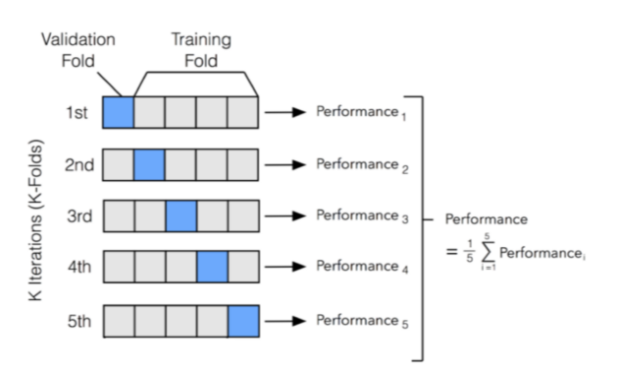
\includegraphics[width=8cm]{images/caprazlama.PNG}\\
	\caption{5-katlı çapraz doğrulama\cite{resim}}
    \label{fig}
\end{figure}
\subsection{Veri Seti}
Bu çalışmada Kaggle sitesinden kalp yetmezliği hastalığı ile ilgili “Heart Failure Prediction Dataset” veri setini temin etmekteyim\cite{veriseti}. Veri setimiz 11 klinik özelliği ve 1 adet çıktı ile kalp hastalığını tespit etmeye çalışmaktadır. Bu öznitelikler aşağıda açıklamaları ile gösterilmektedir.\\
\textbf{Yaş:} Bireyin yaşıdır. Sayısal türde bir öznitelliktir.\\
\textbf{Cinsiyet:} Bireyin cinsiyetidir.\\
\textbf{Göğüs ağrısı tipi:} Bireyin göğüs ağrısı tipidir.(TA: Tipik Angina, ATA: Atipik Angina, NAP: Anjinal olmayan ağrı, ASY: Asemptomatik)\\
\textbf{Dinlenme kan basıncı:}Bireyin kan basınc değeridir ve mm Hg ölçü birimidir.\\
\textbf{Kolestrol:}Bireyin kolestrol değeridir ve mm/dl ölçü birimidir.\\
\textbf{Açlık kan şekeri:} Bireyin kan şekeri değeri [1: if kan şekeri büyükse 120mg/dl, 0:120 den büyük değilse]\\
\textbf{Dinlenme elektrodiyagram:} Bireyin elektrodiyagram sonuçlarıdır.[Normal: Normal, ST: ST-T dalga anormalliği olan T dalgası inversiyonları ve/veya ST elevasyonu veya depresyonu büyükse 0.05 mV), LVH: Estes kriterlerine göre olası veya kesin sol ventrikül hipertrofisini gösteriyor]\\
\textbf{Max kalp hızı:}Bireyin ulaşılan maksimum kalp hızı(60 ile 202 arasında sayısal değer)\\
\textbf{Egzersize bağlı angina:}Bireyin egzersize bağlı angina sonucudur.[Y:Evet, N:Hayır]\\
\textbf{Oldpeak:} Bireyin depresyonda ölçülen ST sayısal değeridir.\\
\textbf{StSlope:}Bireyin zirve egzersiz ST segmentinin eğimidir.[Up: upsloping(eğimli), Flat: flat(düz), Down: dowmsloping(aşağı eğimli)]\\
\textbf{HeartDisease:}Kalp hastası olup olmadığını gösteren sonuc özelliğidir.[1: kalp hastası, 0: değil]

Veri setinin her bir özniteliğinin neler olduğunu gözlemlenmiştir. Bu aşamada yapılacak şey veri setinin sınıf etiketine göre yani hasta olma ve olmama durumları karşılaştırılmalıdır. Burada veri setinin dağılımı gözlemlenmektedir. Çünkü veri setin dengesiz ise modelimiz ne kadar başarılı gözükse de aslında başarılı değildir ve bu yüzden veri setinin dağılımı önem arz etmektedir. Verinin dağılımı Şekil 3'te görülmektedir.
\begin{figure}[htbp]
    \centering
   	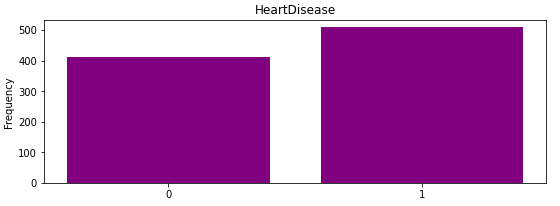
\includegraphics[width=8cm, height=5cm]{images/dagilim.PNG}\\
	\caption{veri setinin dağılım grafiği}
    \label{fig}
\end{figure}
Şekil 3'te de görüldüğü gibi veri setimizdeki dağılım düzgün bir dağılımdır. Bu yüzden bir işlem yapmamıza gerek kalmamıştır. Eğer veri seti dengesiz olsaydı dengesizliği gidermek için bazı işlemler uygulanması gerekmekteydi.
\subsection{Sınıflandırma Problemi Performans Ölçütleri}
Sınıflandırma problemi çıktımızın yani tahmin ettiğimiz değerin ayrık bir veri olduğunda kullanılır. Yani sınıflandırma ayrık verileri tahmin eder. Sınıflandırma algoritmalarının başarısının ölçülmesi için bir kaç metrik vardır. Bunlar modelin ne kadar doğru olduğunu ve başarılı olduğunu tespit etmektedir. İlk inceleyeceğimiz başarı metriğimiz karışıklık matrisi(confusion matrix)'dir. Karışıklık matrisi şekil 'te görülmektedir. Karışıklık matrisinin ne olduğu ve nasıl çalıştığı aşagıda anlatılmıştır.
\begin{figure}[htbp]
    \centering
   	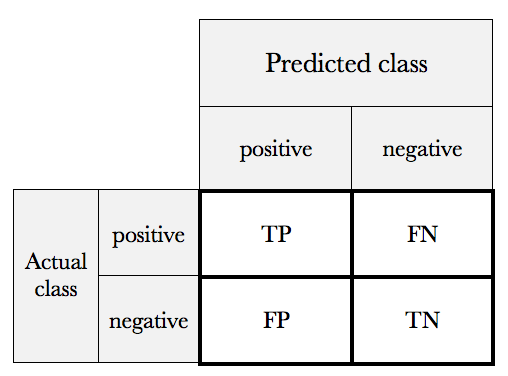
\includegraphics[width=8cm, height=5cm]{images/matris.PNG}\\
	\caption{karışıklık matrisi\cite{confmat}}
    \label{fig}
\end{figure}
Karışıklık matrisi sınıflandırma algoritmalarının başarısını ölçmektedir. Modelin kendisine gelen verileri ne kadarını doğru tahmin etmiş ne kadarını yanlış tahmin etmiş onu göstermektedir. Aşağıda karışıklık matrisinin terimleri açıklanmaktadır.\\\\ 
\textbf{True Negative(TN):} Kişi kalp yetmezliği hastası değilse ve bizde bu kişiye hasta değilsin demişsek hasta olmayan kişiyi doğru tahmin ettiğimiz anlamına gelmektedir.\\
\textbf{True Positive(TP):} Kişi kalp yetmezliği hastasıysa ve bizde ona hastasın dediysek hasta olanı doğru tahmin ettiğimiz anlamına gelmektedir.\\
\textbf{False Negative(FN):} Eğer kişi kalp yetmezliği hastası ise ve biz ona hasta değilsin demişsek hasta olanı yanlış tahmin ettiğmiz anlamına gelir.\\
\textbf{False Positive(FP):} Eğer kişi kalp yetmezliği hastası değilse ve biz ona hastasın demişsek hasta olmayanı yanlış tahmin ettiğimiz anlamına gelmektedir.

Makine öğrenmesinde sınıflandırma problemlerinin başarısını ölçmek için daha birçok metrik vardır. Bunlar tek tek aşağıda açıklanmaktadır.

\textbf{Doğruluk(Accuracy) Skoru:} Modelimizin kaç tane bireyi doğru tahminlediğinin yüzdesel değeridir.Formülü Şekil 5'te görülmektedir.

\begin{figure}[htbp]
    \centering
   	 \Large $Accuracy=\tfrac{TP+FP}{TP+FP+TN+FN}$
	\caption{Accuracy Formülü}
    \label{fig}
\end{figure}

\textbf{Kesinlik(Precision):} Hasta olarak tahmin etmemiz gereken ne kadar kişiyi doğru tahmin ettiğimizi gösteren bir değerdir.Formülü Şekil 6'da görülmektedir.
\begin{figure}[htbp]
    \centering
   	 \Large $Precision=\tfrac{TP} {TP+FP}$
	\caption{Precision Formülü}
    \label{fig}
\end{figure}

\textbf{Duyarlılık(Recall):} kişi hastayken hasta olarak tahmin edilen değerlerin bütün gerçek hasta değerlerine oranını ifade etmektedir.Formülü Şekil 7'de görülmektedir.
\begin{figure}[htbp]
    \centering
   	 \Large $Recall=\tfrac{TP} {TP+TN}$
	\caption{Recall Formülü}
    \label{fig}
\end{figure}

\textbf{F1-Skoru:}Duyarlılık ve kesinlik değelerinin harmonik ortalamasıdır.
\begin{figure}[htbp]
    \centering
   	 \Large $F Score=2\times\tfrac{precision \times recall}{precision+recall}$
	\caption{Recall Formülü}
    \label{fig}
\end{figure}

\textbf{AUC:} AUC ayrılabilirliğin derecesini veya ölçüsünü temsil eder ve ROC eğrisinin altında kalan alandır\cite{auc}. AUC değeri ne kadar yüksek ise modeldeki sınıfları ayırt etme başarısı daha yüksek demektir. Şekil 8'de AUC grafiği temsili görülmektedir.
\begin{figure}[htbp]
    \centering
   	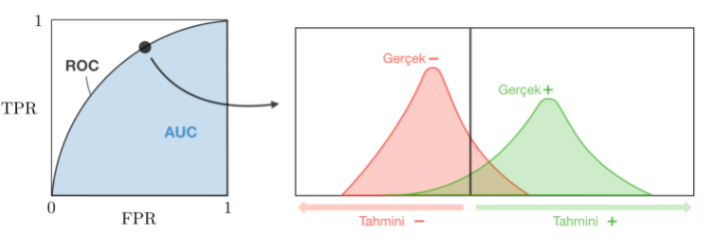
\includegraphics[width=8cm]{images/aucresim.PNG}\\
	\caption{AUC\cite{auc}}
    \label{fig}
\end{figure}

\subsection{Makine Öğrenmesi Modelleri}
Bu alt başlıkta sınıflandırma problemimizde kullandığımız algoritmaların çalışma şekli açıklanmaya çalışılmıştır. Çalışmanın daha iyi anlaşılması için sınıflandırma algoritmalarının çalışma yapısının anlaşılması önemlidir. Kalp yetmezliği teşhisi için K en yakın komşu(K-nearest neighbors) ve yapay sinir ağları(Artificial Neural Network) algoritmaları kullanılmıştır. İlk olarak K en yakın komşu algoritması açıklamaya çalışılmıştır.
\subsubsection{K en yakın komşu algoritması(KNN)}
KNN algoritmasında bir K değeri belirlenmektedir ve yeni gelen veri en yakın K komşusuna bakarak hangi sınıfa dahil olacağı belirlenmektedir.K en yakın komşu algoritması hem sınıflandırma da hem de regresyon problemlerinde kullanılabilmektedir. Biz bu çalışmda çıktımız ayrık veri olduğu için KNN'i sınıflandırma amaçlı kullanılacaktır. Yeni gelen veri en yakın K komşusuna bakarak en çok olan sınıfa atanır. KNN çalışma Şekil 10'da gösterilmiştir.
\begin{figure}[htbp]
    \centering
   	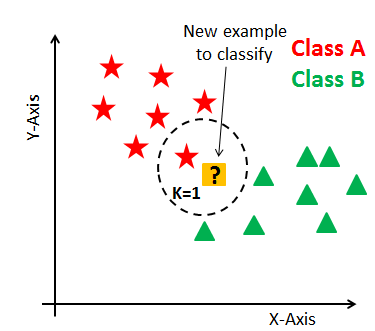
\includegraphics[width=8cm]{images/knnresim.PNG}\\
	\caption{K nearest neighbors(KNN) algoritması\cite{resimknn}}
    \label{fig}
\end{figure}
Bu çalışmada önerilen KNN modeli oluşturulurken modelin başarısının artması için en optimum K değerinin belirlenmesi gerekmektedir. Bu yüzden hiperparametre optimizasyonu yapmak için GridSearchCV algoritması kullanılmıştır. GridSearchCV algoritması ile en iyi K değerinin bulunmasının amaçlanmıştır. Bir K liste değeri vererek en iyi K değeri bulunduktan sonra en optimum K değeri ile model yeniden oluşturulması amaçlanmıştır.
\subsubsection{Yapay Sinir Ağları(ANN)}
Artificial Neural Network(ANN) algoritması çalışma şekli açıklanmaya çalışılmıştır.ANN insan beyninin çalışma mantığından esinlenmiş ve öğrenme sürecinin matematiksel olarak modellenmesi temeline dayanmaktadır.ANN girdi katmanı,gizli katman ve çıkış katmanları bulunmaktadır.
Bu çalışmamızda belirli hiperparametreler vererek bu hiperparametreler içerisindeki modelimzde en fazla başarı gösteren hiperparametre kombinasyonun bulunması amaçlanmıştır.\\
Bu aşamada da hiperparametre optimizasyonu için GridSearchCV algoritması kullanılmıştır. Ve bu hiperparametre optimizasyonu sonucu elimizde 1 giriş katmanı,32,16,16 nöronlu dense tipinde gizli katman,1 gizli katmandan oluşan, her katmanın sonunda 0.25 dropout,epoch değeri 100 , batchsize değeri 64 ,sigmoid aktvasyonuna ve adam optimizasyonuna sahip bir model bir ANN modeli önerilmiştir.

\subsection{LİTERATÜR TARAMASI}
Bu kısımda kalp yetmezliği hastalığını tespit eden makine öğrenmesi tabanlı projeler incelenip rapor edilmiştir ve deneysel sonuçlar kısmında karşılaştırmalı olarak analiz edilecektir. Literatürde Lojistik regresyon, rastgele orman(random forest),ekstra ağaçlar(Extra tree) ve karar ağaçları(decision tree) vb.
algoritmalar görülmüştür.

Mustafa Coşar ve Emre Deniz(2021) kalp yetmezliği teşhisi için 3 farklı algoritmalar kullanmışlardır.Bunlar Lojistik regresyon, random forest ve KNN algoritmalarını kullanarak modeller karşılaştırılmıştır. Ve kalp yetmezliği hastalığını teşhis etmede \%85 ile lojistik regresyon olmuştur ve sonuç rapor edilmiştir.

Prasanta Kumar Sahoo ve Pravalika Jeripothula(2020) kalp yetmezliği teşhisi için 2 farklı algoritma kullanılmıştır. Bunlar Decision Tree ve SVM algoritmaları kullanılmıştır.Ve kalp yetmezliği hastalığını teşhis etmede \%85.2 ile SVM algoritması olduğu rapor edilmiştir.

Ashok Kumar Dwivedi(2018) kalp yetmezliği teşhisi için ANN, SVM, Lojistik regresyon,KNN, classfication tree ve Navie bayes algortimaları kullanılmıştır. Ve kalp yetmezliği hastalığını teşhis etmede \%85 ile Lojistik regresyon olmuştur ve sonuç rapor edilmiştir.


\section{DENEYSEL SONUÇLAR VE TARTIŞMA}
Bu çalışmada ANN ve KNN sınıflandırma algoritmaları kullanılarak model eğitilmiştir.Ve bu model kullanılarak bireylerin kalp hastalığı tespit edilmiştir.Tüm modellerimiz için en iyi hiperparametre kombinasyonunu bulduktan sonra modeller yeniden oluşturulmuştur.Ve tüm modellerimize 10 katlı çapraz doğrulama ile modelin başarısı sınanmıştır. Bu çalışmada 2.40 GHz Intel Core i5-9300H işlemci, 16GB RAM, 1TB SSD bellek ve windows10 işletim sistemine sahip bir sistem ve Anaconda dağıtımı üzerinden jupyter lab
kullanılarak Python programlama dili kullanılmıştır. Bu kısımda modelleri karşılaştırılmalı olarak simulasyon sonuçları sunulmaktadır.
\subsection{Simülasyon Sonuçları}
Deneysel sonuçlarda, kalp hastalığını tespit eden doğrulanmış modellerimiz arasında en iyi başarıyı ANN sınıflandırıcı göstermiştir.Modellerimizi doğruluk(accuracy),kesinlik(precision),duyarlılık (recal), F1 skoru ve AUC skoru değerleri ile karşılaştırılmıştır.Modellerin bu değerleri Şekil 11'de görülmektedir.
\begin{figure}[htbp]
    \centering
   	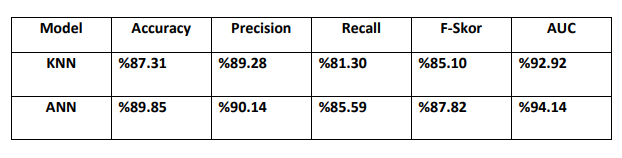
\includegraphics[width=8cm]{images/sonuc.PNG}\\
	\caption{Performans karşılaştırma ölçüt skorları}
    \label{fig}
\end{figure}
10 kat çapraz doğrulama tekniği ile oluşturulan modeller arasında kalp yetmezliği hastalığını teşhis eden iyi sınıflandırıcı algoritması ANN modelidir. ANN modeli KNN modeline göre daha iyi sonuçlar vermektedir. 
DEneysel sonuçları sonucu elde edilen başarı metriklerini tabloda göstermiştik.Ama bence her zaman bir grafik üzerinde görmek her zaman daha anlaşılır olacaktır.Şekil 12'de sınıflandırıcı algoritmalar için belirlediğimiz metrikleri grafiğe aktarılmış hali bulunmaktadır.
\begin{figure}[htbp]
    \centering
   	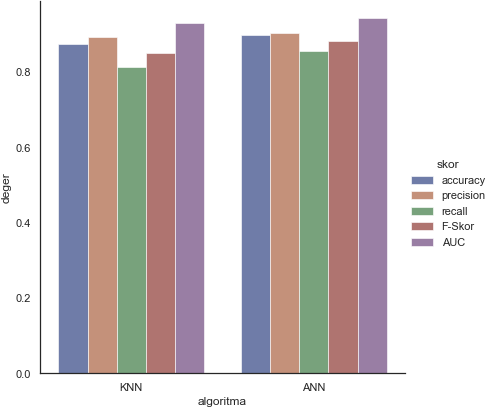
\includegraphics[width=8cm]{images/sonucgrafik.PNG}\\
	\caption{Performans karşılaştırma ölçüt skor grafiği}
    \label{fig}
\end{figure}
Modellerimizin başarı metriklerinin dağılımını görmek için belirlen başarı metriklerinin 10 katlı çapraz doğrulama sonrası belirlediğimiz başarı metriklerinin standart sapması Şekil 13'te görülmektedir.
\begin{figure}[htbp]
    \centering
   	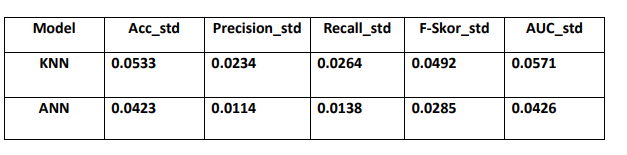
\includegraphics[width=8cm]{images/sonucstd.PNG}\\
	\caption{Performans karşılaştırma ölçüt standart sapma değerleri}
    \label{fig}
\end{figure}
Bu standart sapma değerinin düşük olması dağılımın ortalamadan fazla uzaklaşmadığı anlamına gelektedir. Bu da istenilen bir durumdur.Burada da ANN modeli KNN modeline göre daha düşük standart sapma değerlerine sahip olduğu görülmektedir.
Modelimizdeki ANN modeli ile literatür taraması sonucu elde edilen modeller ile karşılaştırılması önem arz etmektedir. Bundan sonraki kısımda en iyi ANN modeli ile karşılaştırma yapılacaktır. Şekil 14'te modelimiz ile literatür taramasındaki her bir çalışmanın modeli ile karşılaştırmalar yapılmıştır.
\begin{figure}[htbp]
    \centering
   	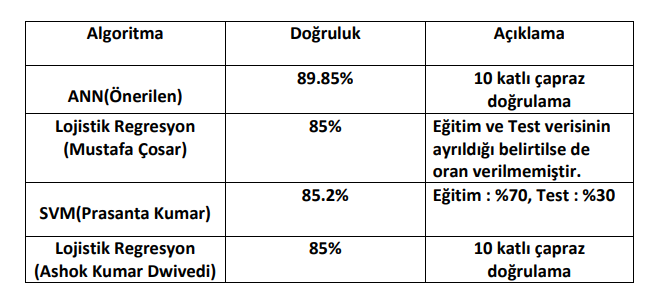
\includegraphics[width=8cm]{images/karsilastirmaresim.PNG}\\
	\caption{Literatürdeki diğer modellerle performans karşılaştırma}
    \label{fig}
\end{figure}

\section{SONUÇ}
Bu çalışmada kalp yetmezliği hastalığının belirlenmesi için makine öğrenmesi algoritmalarını kullanrak kalp hastalığını belirleyen en iyi model bulunmak amaçlanmıştır.Bakılan algoritmalar içerisinde en iyi başarı gösteren model \%89.85 ile ANN modeli olmuştur. Literatür taraması sonrasında en başarılı olan mdeol yine bizim ANN modelimiz olmuştur.
Kalp yetmezliği teşhisi için, veri setinde aykırı değerlerin silinmesi veya daha fazla veri ile desteklenmesi sonucu daha başarılı modeller çalışmalar yapılabilir.Ayrıca en iyi öznitelikler seçilerek de modelin başarı oranının artırılmasına yönelik çalışmalar yapılabilir.

\printbibliography
\end{document}

